\documentclass[10pt,a4paper]{article}
\usepackage[latin1]{inputenc}
\usepackage{amsmath}
\usepackage{amsfonts}
\usepackage{amssymb}
\usepackage[pdftex]{graphicx}
\usepackage{float}

\begin{document}
\title{The Kuramoto-Sivashinsky Equation}
\author{Anders, Elisabeth og Espen}

\maketitle



\begin{abstract}
This is the abstract. Write smart things here.
\end{abstract}

%\begin{figure}[H]
%\centering
%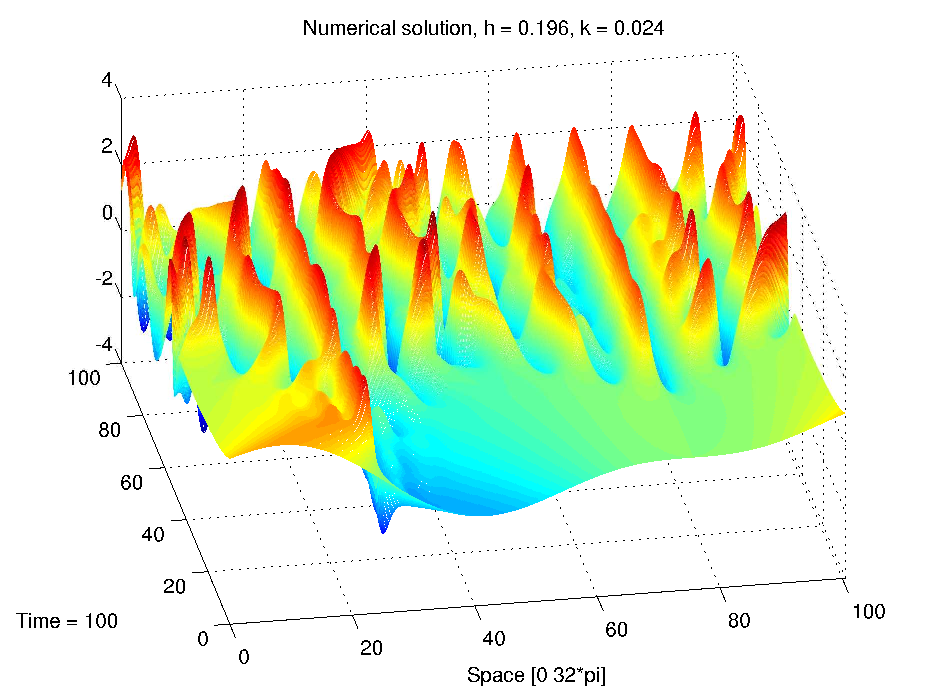
\includegraphics[scale=0.5]{PDFs/IMEX/KS_plot_surface.pdf}
%\end{figure}


\section*{Introduction}
The Kuramoto-Sivashinsky equation,
\begin{equation}
\label{KSeq}
u_t + u_{xx} + u_{xxxx} + uu_{t} = 0 
\end{equation}
written in integral form as
\begin{equation*}
h_t + h_{xx} + h_{xxxx} + \frac{1}{2}h^2_x = 0, u = h_x 
\end{equation*}
is one of the simplest partial differential equations that exhibits complicated dynamics in both time and space, which is why the equation has been the attention for a lot of research. The equation was developed by two scientists at the same time in 1977 \cite{development}. Gregory Sivashinsky determined an equation for a laminar flame front, while Yoshiki Kuramoto modeled a diffusion-induced chaos using the same equation. Because of this, the equation is named Kuramoto-Sivashinsky. The KS-equation also models the motion of a fluid going down a vertical wall, e.g. solitary pulses in a falling thin film. \cite{trivia}

The reason for the complex behaviour comes from the second- and fourth-order derivatives in \eqref{KSeq}. While the second-order term acts as an energy source and has a destabilizing effect, the fourth-order term has a stabilizing effect. In addition to this, the nonlinear term transfers energy from low to high wave numbers. \cite{stabil} The KS-equation is a stiff equation, i.e. an equation where numerical methods for solving it are numerically unstable, unless the step size is extremely small. $u_{xxxx}$ is the main reason for this as it leads to rapid variation in the solution.


%Of particular interest is the case when the stiff terms are linear, which is the case of the %Kuramoto–Sivashinsky equation. Under these conditions, it may be extremely advantageous to %split the equations into its stiff and nonstiff components, and treat each of them %separately. In particular, the nonlinear, nonstiff terms are integrated using a suitable %explicit scheme, whereas the linear, stiff terms and integrated using and implicit scheme
%http://raphael.mit.edu/lcf_jp_JCP08.pdf


%http://en.wikipedia.org/wiki/Stiff_equation

%cite trivia: http://www.sciencedirect.com/science/article/pii/S0307904X11004082


%cite something: http://www.naturalspublishing.com/files/published/ed38fj6n3xt187.pdf



\begin{thebibliography}{9}

\bibitem{development}
Scott Arthur Gasner, Fall 2004,
\emph{Integrating the Kuramoto-Sivashinsky equation: A simulation of the hopping state}
http://terminus.sdsu.edu/thesis\_repository/ScottGasner\_2004\_Fall\_MS\_Comp\_Sci.pdf, 03/31-2014

\bibitem{trivia}
Mehrdad Lakestani and Mehdi Dehghan, February 2012,
\emph{Numerical solutions of the generalized Kuramoto-Sivashinsky equation using B-spline functions},
http://www.sciencedirect.com/science/article/pii/S0307904X11004082, 03/31-2014

\bibitem{stabil}
Marjan Uddin and Sardar Ali, January 2013,
\emph{RBF-PS method and Fourier Pseudospectral method for solving stiff 
nonlinear partial differential equations},
http://www.naturalspublishing.com/files/published/ed38fj6n3xt187.pdf, 03/31-2014


\end{thebibliography}


\end{document}